\chapter{Motor Actuation}

Once the system specifications were decided, multiple motor suppliers in Pakistan were contacted to initiate procurement of AC servo motors. However, most of them could not meet project requirements, with issues such as unreasonably long lead times, inappropriate motor frames and power ratings, and exorbitant prices. Fortunately, one supplier offered Yaskawa Sigma-5 AC servo motors at reasonable rates, along with compatible drives and cabling. Considering that the Sigma-5 series is targeted toward precision motion control applications and Yaskawa's proprietary motor sizing software \textit{SigmaSelect} was available on their website, Yaskawa was selected as the motor vendor. Thus, all subsequent sizing was done using \textit{SigmaSelect}.

\begin{figure}[H]
    \centering
    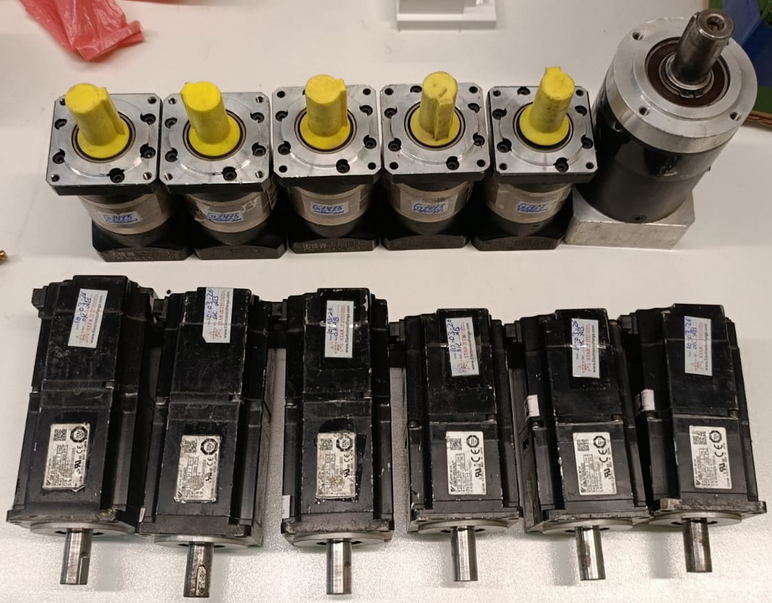
\includegraphics[width=0.8\textwidth]{figures/motors_gearboxes}
    \caption{Procured Yaskawa Sigma-5 servo motors and drives.}
    \label{fig:motors_gearboxes}
\end{figure}

\section{Kinematic Motion Profile}

To define a common baseline for all axes, a trapezoidal motion profile with S-curve smoothing was utilized. This does not represent the final trajectory; it is developed to a point where motor selection can be confirmed, with further refinement of exact parameters not affecting sizing outcome meaningfully, as determined by experimentation within the software. The hard constraints are a \SI{3.0}{m} travel distance for the linear axes and $180\degree$ for yaw, and a total traversal time of \SI{10}{s} so that a full cycle can complete within \SI{20}{s}, leaving the remaining time for picking and placing. The remaining profile parameters were selected as follows and are subject to minor refinement:

\begin{itemize}
    \item \textbf{Total Distance ($D$):} \SI{3.0}{m} or \SI{180}{\degree} 
    \item \textbf{Total Time ($t_\text{tot}$):} \SI{10.0}{s}
    \item \textbf{Acceleration Time ($t_a$):} \SI{1.0}{s}
    \item \textbf{Deceleration Time ($t_d$):} \SI{1.0}{s}
    \item \textbf{Jerk Time ($t_j$):} \SI{0.5}{s}
\end{itemize}

The acceleration and deceleration times of \SI{1.0}{s} were selected to keep peak acceleration within the motor's rated torque envelope without requiring oversized motors. The jerk time of \SI{0.5}{s} ensures a smooth S-curve transition at the boundaries of the acceleration region, so that the commanded jerk remains finite and the resulting motion does not excite mechanical resonances. These values were refined iteratively in \textit{SigmaSelect}: shorter acceleration times demanded peak torques exceeding the motor's intermittent rating, while longer times consumed too much of the \SI{10}{s} traversal window.

This results in a peak constant velocity of:

\begin{equation}
    V_\text{max} = \frac{D}{t_\text{tot} - \dfrac{t_a + t_d}{2}} 
    = \frac{3.0}{10.0 - 1.0} \approx \SI{0.333}{m/s}
\end{equation}

\begin{figure}[H]
    \centering
    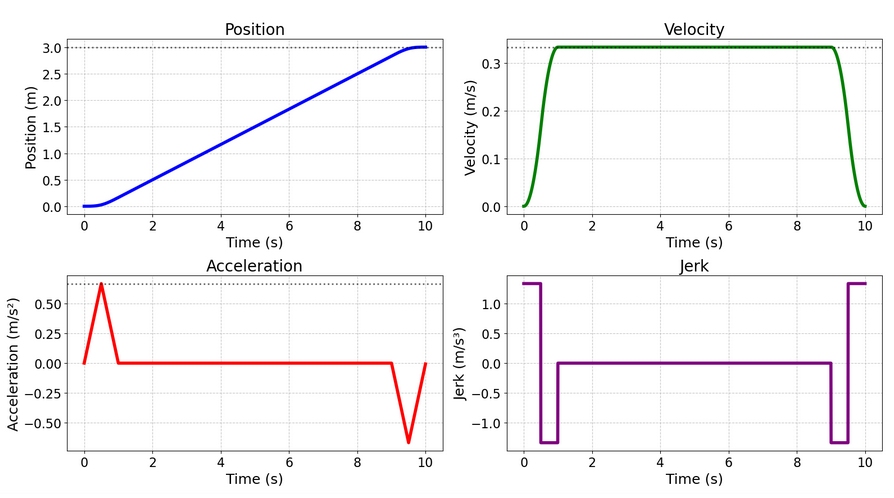
\includegraphics[width=0.95\textwidth]{figures/motor_sizing_graphs}
    \caption{Trapezoidal motion profile with smoothing as defined in SigmaSelect.}
    \label{fig:motion_profile}
\end{figure}

\section{Moving Mass Estimation}

For \textit{SigmaSelect} to calculate load and peak torques, the total moving mass of the gantry was estimated through a breakdown of each subsystem that moves on the robot. This means that the X-axis drive motors, which are bolted to the frame and are static, are not part of the moving mass. The breakdown is given in Table~\ref{tab:mass_budget}. All component masses were obtained from manufacturer catalogues and vendor specifications; where exact data was unavailable, values were rounded up to maintain a conservative estimate.

\begin{table}[H]
    \centering
    \begin{tabular}{@{}llcp{4.5cm}@{}}
        \toprule
        \textbf{Subsystem} & \textbf{Component} & \textbf{Mass (kg)} & \textbf{Notes} \\
        \midrule
        \multirow{4}{*}{\shortstack[l]{\textbf{X-Axis}\\\textbf{Bridge}\\(\SI{60.0}{kg})}}
            & Main Steel Beam       & 30.0 & $80\times80\times4$\,mm SHS, \SI{3}{m} span \\
            & Y-Axis Linear Rails   & 16.0 & Two 20\,mm profile rails \\
            & End Plates            & 10.0 & Two \SI{10}{mm} steel plates \\
            & Hardware \& Fasteners &  4.0 & Bolts, T-nuts, brackets \\
        \midrule
        \multirow{4}{*}{\shortstack[l]{\textbf{Y-Axis}\\\textbf{Carriage}\\(\SI{10.0}{kg})}}
            & Motor \& Gearbox      &  2.8 & 400\,W Sigma-5 + planetary gearbox \\
            & Carriage Plate        &  5.0 & Machined steel mounting plate \\
            & Linear Bearing Blocks &  1.2 & Four 20\,mm profile blocks \\
            & Cable Carrier         &  1.0 & Drag chain, wiring, pneumatics \\
        \midrule
        \multirow{5}{*}{\shortstack[l]{\textbf{Z-Axis}\\\textbf{Assembly}\\(\SI{45.0}{kg})}}
            & Dual Motors \& Gearboxes  &  7.2 & Two 200\,W Sigma-5 + gearboxes \\
            & Stationary Drive / Shafts & 10.0 & Cross-shafts + mounting plates \\
            & Vertical Cuboid Structure & 11.5 & \SI{2.5}{m} steel chassis \\
            & 2.5\,m Racks \& Rails     & 11.7 & Mod.\,2 racks + 20\,mm profile rails \\
            & Yaw Drive \& End Effector &  4.6 & 200\,W servo + suction head \\
        \midrule
        \textbf{Payload}
            & Microwave Unit & 40.0 & Dawlance spec., with safety factor \\
        \midrule
        \textbf{Total ($M_\text{moving}$)} & & \textbf{155.0} & Sum of all dynamic components \\
        \bottomrule
    \end{tabular}
    \caption{Moving mass budget.}
    \label{tab:mass_budget}
\end{table}

On top of the component-level estimates, a 10\% safety factor was applied to yield $M_\text{total} = \SI{170}{kg}$ for all sizing. This safety factor accounts for real-world variation such as asymmetric loading, belt tensioning forces, and potential future payload changes, and reflects the priority of safety over cost as expressed by Dawlance.

\section{Load Parameters}

The total moving mass of \SI{170}{kg} is distributed differently across the axes, because each motor only drives the components that move along its own axis.

The X-axis is driven by two synchronised motors, one on each side of the bridge. If the bridge is assumed to be rigid and symmetric, then the moving mass is divided equally to be \SI{85}{kg} per motor. When the Y-axis carriage is positioned asymmetrically (i.e., at one end of the bridge rather than centred), the load distribution between the two X-axis motors becomes unequal. The four-block carriage configuration described in Chapter~4 mitigates this by distributing the reaction forces across a wide stance, but the sizing uses the symmetric \SI{85}{kg} figure as a conservative average.

The Y-axis motor drives everything that moves along the Y rail: the Y-axis carriage (\SI{10}{kg}), the Z-axis assembly (\SI{45}{kg}), and the payload (\SI{40}{kg}), plus the 10\% safety factor applied proportionally. The X-axis bridge (\SI{60}{kg}) does not move along the Y direction and is therefore excluded. This gives a Y-axis driven mass of:
\[
M_Y = M_\text{total} - M_\text{bridge} = 170 - 60 = \SI{110}{kg}
\]

The Z-axis supports the vertical structure (\SI{11.5}{kg}), racks and rails (\SI{11.7}{kg}), the yaw drive and end-effector (\SI{4.6}{kg}), and the payload (\SI{40}{kg}), with the safety factor applied. After excluding the Z-axis motors, cross-shafts, and mounting plates (which are fixed to the Y-axis carriage and do not translate vertically), the suspended mass is approximately \SI{70}{kg}, divided between two synchronised Z-axis motors at \SI{35}{kg} each.

The yaw axis motor experiences only the rotational inertia of the payload, as the yaw shaft and bearing assembly contribute negligible inertia relative to the microwave.

\section{Transmission Parameters}

Before presenting the specific values, it is useful to define the key transmission parameters that \textit{SigmaSelect} requires. For belt drives, the critical parameters are the belt pitch (tooth spacing in mm) and the pulley tooth count, which together determine the pitch diameter and hence the linear displacement per motor revolution. For rack-and-pinion drives, the analogous parameters are the module and tooth count: module is the ratio of the pitch diameter to the number of teeth, expressed in millimetres, so that Module~2 means each tooth occupies \SI{2}{mm} of pitch diameter. In both cases, the gear ratio of the planetary gearbox between the motor and the transmission determines how much the load inertia is reduced as seen by the motor.

All three linear axes use a 20:1 planetary gearbox. The gear ratio was determined by sweeping ratios from 5:1 to 50:1 in \textit{SigmaSelect}; 20:1 was the lowest ratio that kept the reflected inertia ratio below the drive's 10:1 tuning limit while maintaining operating speed within rated RPM. This was also the lowest ratio available through the motor vendor. The 20:1 ratio reduces the load inertia reflected to the motor shaft by a factor of $G^2 = 400$. The yaw axis uses a 160:1 planetary drive gearbox due to the exceptionally large rotational inertia of the microwave, as discussed in Section~\ref{sec:yaw_sizing}.

The X and Y axes use an HTD\,8M synchronous belt with \SI{8}{mm} pitch, selected for its availability in the local market and its rated load capacity exceeding the peak belt tension for these axes. Since the minimum recommended tooth count for a pulley is 17 and exceeding 20 teeth increases the effective pitch diameter --- which, in turn, worsens the inertia ratio --- a 20-tooth drive pulley was selected. With these parameters, the pitch diameter is $\frac{P \cdot Z}{\pi} = \frac{8 \times 20}{\pi} \approx \SI{50.9}{mm}$. A conservative mechanism efficiency of $\eta_\text{mech} = 0.90$ (HTD drives normally achieve 0.95--0.98) and a friction coefficient of $\mu = 0.01$ (recirculating linear guides normally achieve 0.005) complete the parameter selection for the X and Y axes.

For the Z-axis rack-and-pinion, Module~2 was selected for its adequate tooth strength for industrial loads, and 20 teeth for the pinion following the same logic as the pulley tooth count. The yaw axis is directly coupled with the payload through the planetary drive and requires no additional transmission parameter selection.

\section{X and Y Axes Sizing Results}

\textit{SigmaSelect} evaluated the \SI{400}{W} Yaskawa Sigma-5 motor on both axes. In both cases, the software confirmed that the motor selection satisfied the motion profile with significant margin. The inertia ratio was below 10:1 with headroom, so that the servo drive can be tuned for stable positioning --- critical for industrial robotics applications. Peak and continuous torque demands are well within the motor's rated limits, as well as the operating and maximum speeds.

It should be noted that the Y-axis was initially sized with a driven mass of \SI{100}{kg}; upon review, the correct value is \SI{110}{kg} as derived in Section~6.3. However, examination of the SigmaSelect results in Figure~\ref{fig:y_sigma} shows that the application torque of \SI{0.243}{Nm} is only 19\% of the motor's rated torque of \SI{1.27}{Nm}, and the inertia ratio of 9.45 remains below the 10:1 limit. The additional \SI{10}{kg} increases the reflected inertia and required torque marginally, and the motor continues to satisfy all sizing criteria with adequate margin.

\begin{figure}[H]
    \centering
    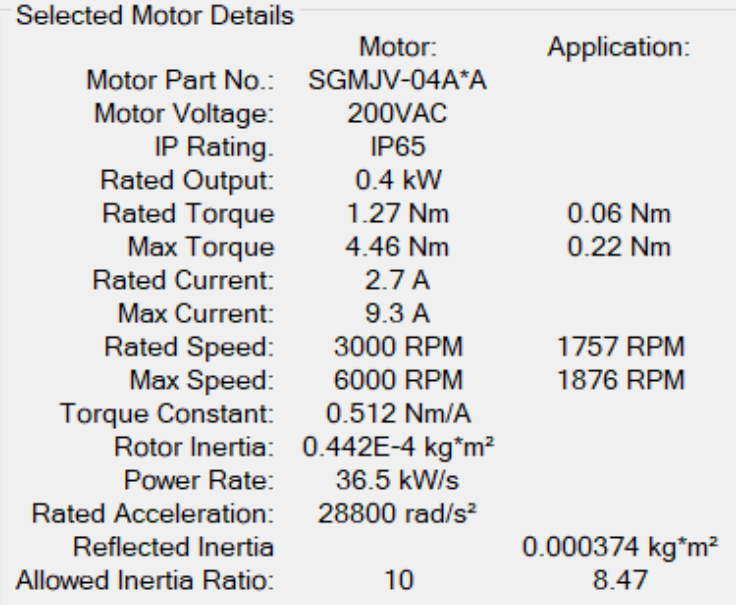
\includegraphics[width=0.8\textwidth]{figures/x_sigma}
    \caption{SigmaSelect sizing results for the X-axis 400\,W Yaskawa Sigma-5 motor.}
    \label{fig:x_sigma}
\end{figure}

\begin{figure}[H]
    \centering
    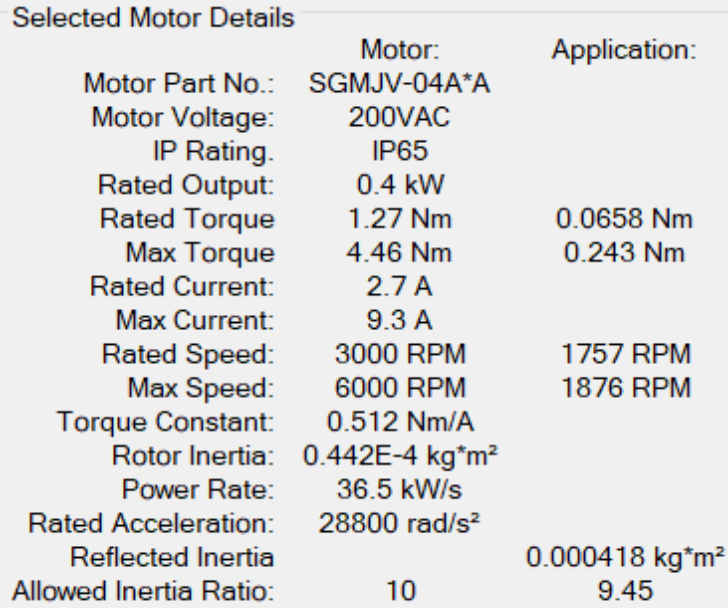
\includegraphics[width=0.8\textwidth]{figures/y_sigma}
    \caption{SigmaSelect sizing results for the Y-axis 400\,W Yaskawa Sigma-5 motor.}
    \label{fig:y_sigma}
\end{figure}

\section{Z-Axis Sizing Results}

Unlike the horizontal axes where gravity acts perpendicular to the direction of travel, the Z-axis motors must continuously generate torque to support the suspended mass against gravity, even when stationary. This makes the Z-axis the most demanding linear axis despite its reduced load. Two \SI{200}{W} Sigma-5 motors are used, one for each rack, with a $90\degree$ inclination angle; with the aforementioned gearbox, \textit{SigmaSelect} confirmed that the motor can satisfy the trajectory with torque and speed within rated limits and the inertia ratio below 10:1.

\begin{figure}[H]
    \centering
    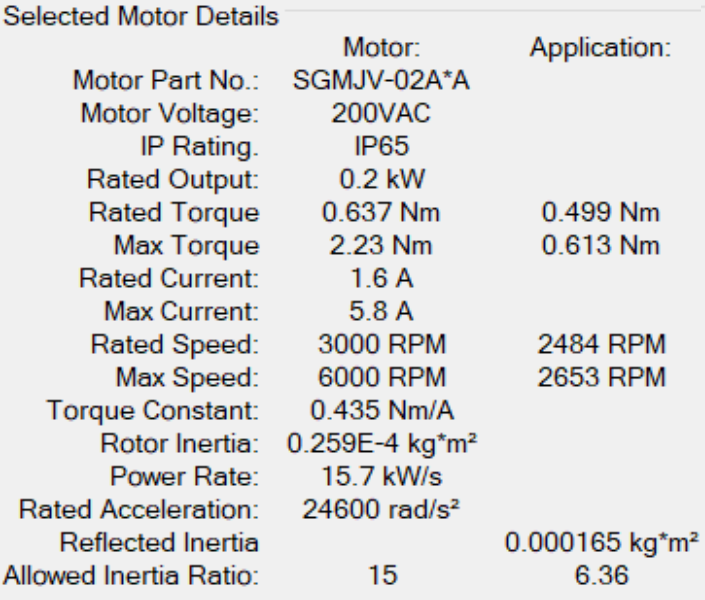
\includegraphics[width=0.8\textwidth]{figures/z_sigma}
    \caption{SigmaSelect sizing results for the Z-axis 200\,W Yaskawa Sigma-5 motor.}
    \label{fig:z_sigma}
\end{figure}

\section{Yaw Axis Sizing}
\label{sec:yaw_sizing}

This axis rotates the end-effector to orient the microwave, which presents a unique problem: modelling the MWO DW-162-HZP (their largest unit) as a rotating table with its physical dimensions yields a moment of inertia of $\approx \SI{2.12}{kg.m^2}$, which is large enough to warrant an extremely high gear reduction. The gear ratio was determined by consultation with the supplier and iterative sizing in \textit{SigmaSelect}; a 160:1 planetary drive reducer was selected with a \SI{200}{W} Sigma-5 motor, which reduces the reflected inertia to within the drive's tuning envelope.

\begin{figure}[H]
    \centering
    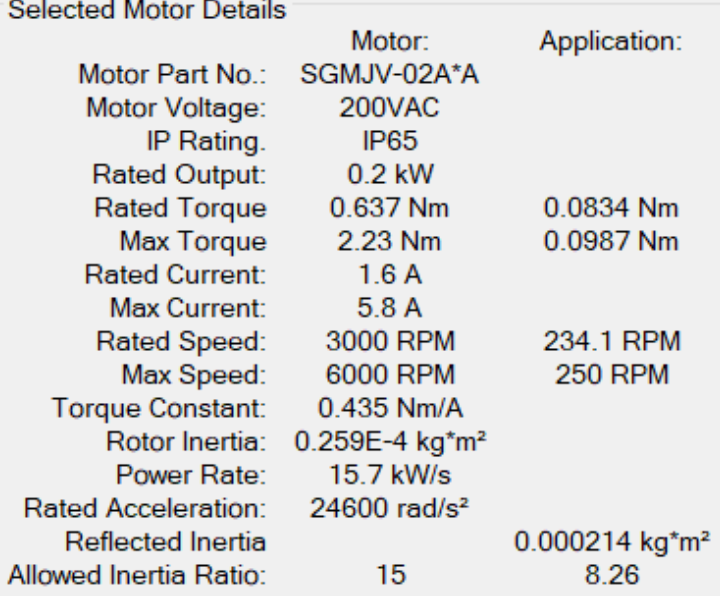
\includegraphics[width=0.8\textwidth]{figures/yaw_sigma}
    \caption{SigmaSelect sizing results for the yaw-axis 200\,W Yaskawa Sigma-5 motor with 160:1 planetary drive reducer.}
    \label{fig:yaw_sigma}
\end{figure}

\section{Motor Selection Summary}

The final motor selection for all axes is summarised in Table~\ref{tab:motor_summary}.

\begin{table}[H]
    \centering
    \begin{tabular}{@{}lcccc@{}}
        \toprule
        \textbf{Axis} & \textbf{Motor} & \textbf{Quantity} 
        & \textbf{Gear Ratio} & \textbf{Drive Mechanism} \\
        \midrule
        X & 400\,W Sigma-5 & 2  & 20:1 planetary & HTD 8M belt \\
        Y & 400\,W Sigma-5 & 1               & 20:1 planetary & HTD 8M belt \\
        Z & 200\,W Sigma-5 & 2 & 20:1 planetary & Mod.\,2 rack \& pinion \\
        Yaw & 200\,W Sigma-5 & 1             & 160:1 planetary drive & Direct output shaft \\
        \bottomrule
    \end{tabular}
    \caption{Final motor and transmission selection across all gantry axes.}
    \label{tab:motor_summary}
\end{table}